\documentclass[12pt,a4paper]{report}

% === PACKAGES ===
\usepackage[utf8]{inputenc}
\usepackage[T1]{fontenc}
\usepackage{setspace}
\usepackage{geometry}
\usepackage{apacite}
\usepackage{graphicx}
\usepackage{titlesec}
\usepackage{fancyhdr}
\usepackage{newtxtext,newtxmath} % Times New Roman font
\usepackage[utf8]{inputenc}
\usepackage{gensymb}
\usepackage{float}


%%\usepackage{textgreek}

% === PAGE SETTINGS ===
\geometry{margin=1in}
\onehalfspacing
\pagestyle{fancy}
\fancyhf{}
\fancyhead[L]{\leftmark} % Chapter title in header
\fancyfoot[C]{\thepage}
\renewcommand{\headrulewidth}{0.4pt}
\renewcommand{\footrulewidth}{0.4pt}

% === SECTION NUMBERING ===
\titleformat{\chapter}{\bfseries\large}{\thechapter.}{1em}{}

\renewcommand{\thesection}{\thechapter.\arabic{section}}
\titleformat{\section}{\bfseries\normalsize}{\thesection}{1em}{}

\renewcommand{\thesubsection}{\thesection.\arabic{subsection}}
\titleformat{\subsection}{\bfseries\normalsize}{\thesubsection}{1em}{}



% === TITLE PAGE ===
\begin{document}
	
	\begin{titlepage}
		\centering
		{{\small \textbf {\underline{Homepaper Submission I \& II}}\par}}
		\vspace{0.3cm}
		{\Large \textbf {\underline{Design of a 20,000 TPA of 2-Hydroxyethyl Methacrylate}}\par}
		\vspace{0.5cm}
		
		{\it submitted to the\par}
		\vspace{0.4cm}
		
		{\large\textbf{INSTITUTE OF CHEMICAL TECHNOLOGY, MUMBAI}\par}
		\vspace{0.2cm}
		
		{\it for Partial fulfillment of the degree of\par}
		\vspace{0.2cm}
		
		{\large Bachelors of Chemical Engineering\par}
		{\large (Semester VII)\par}
		\vspace{0.5cm}
		
		{\large by\par}
		\vspace{0.3cm}
		
		{\Large Nidhi Kulkarni\par}
		{\large 22CHE142\par}
		
		\vspace{1cm}
		
		% ---- Insert Institute Logo ----
		
\includegraphics[width=0.3\textwidth]{figures/ictlogo.jpg}\par
		% Replace 'logo.png' with your actual file name in the same folder.
		
		\vspace{1cm}
		
		{\large Institute of Chemical Technology, Mumbai\par}
		\vspace{0.2cm}
		
		{\small (University Under Section 3 of UGC Act 1956;\par}
		{Elite Status and Centre of Excellence, Government of Maharashtra)\par}
		
		\vspace{1cm}
		
		
		
		{\large December 2025\par}
		
		\vfill
		\begin{flushright}
			\textbf{VGG} \\ % Replace ABC with supervisor's initials
		\end{flushright}
	\end{titlepage}
	
	
	% === INDEX ===
	\tableofcontents
	\newpage
	\listoffigures
	\addcontentsline{toc}{chapter}{List of Figures}
	\newpage

\chapter{Introduction}
2-Hydroxyethyl Methacrylate, abbreviated as \textbf{HEMA}, is a hydroxy ester of methacrylic acid. It
is a monomer that is used to make hydrogels used in making UV cured coatings and adhesives.
The polymer (poly Hydroxyethyl Methacrylate or \textbf{pHEMA}) is used to make hydrogels and
contact lenses, and are used for drug delivery in biomedical fields. Since the monomer
polymerizes quite easily, hydroquinone or methoxyphenol are added as inhibitors.

\section{Product Definitions and properties}
Name : 2-Hydroxyethyl Methacrylate
fig1
\\ Molecular formula: C6H10O3
\\ Appearance: Colourless, viscous liquid
\\ CAS No: 868-77-9
\\ IUPAC name: 2,2-hydroxy,ethyl-methacrylate
\\ Other names: 2-hydroxyethyl 2-methylprop-2-enoate, Glycol methacrylate, and ethylene glycol
methacrylate, Glycol mono-methacrylate

\begin{table}[h]
	\centering
	\renewcommand{\arraystretch}{1.5}
	\begin{tabular}{|l|l|}
		\hline
		\textbf{Property} & \textbf{Value} \\
		\hline
		Molecular Weight & 130.14 g/mol \\
		\hline
		Density (@ 20$^\circ$C) & 1.07 g/cm$^3$ \\
		\hline
		Melting point & -12 $^\circ$C \\
		\hline
		Boiling point (@1 atm) & 205 $^\circ$C \\
		\hline
		Flash point (@1 atm) & 107 $^\circ$C \\
		\hline
		Solubility in water & Completely miscible \\
		\hline
		Vapor pressure (@ 20$^\circ$C) & 20 Pa \\
		\hline
	\end{tabular}
	\caption{Physical properties}
	\label{tab:hysteresis}
\end{table}

\section{Hazards and Toxicity}
Signal word: Warning.
\\ Hazard statements: Causes skin irritation. May cause an allergic skin reaction. Causes serious
eye irritation
\\ Precautionary statements: 
\\ Prevention: P261 Avoid breathing mist or vapors. P264 Wash skin thoroughly after handling. P280 Wear protective gloves/ eye protection/ face protection.
Response: P333 + P313 If skin irritation or rash occurs: Get medical advice/ attention. P337 +
P313 If eye irritation persists: Get medical advice/ attention. P362 + P364 Take off contaminated
clothing and wash it before re-using.

\section{Uses of HEMA}
The industrial and biomedical applications of HEMA encompass
a broad spectrum due to its versatile chemistry and properties. HEMA’s high hydrophilicity and
polymerizability make it indispensable in developing materials where mechanical strength,
biocompatibility, and aqueous interaction are critical.

\subsection{Industrial applications}
	\begin{enumerate}
		\item {Synthesis of coating resins for automotive, architectural, and paper industries}
		\item {Production of advanced adhesives and sealants}
		\item {Textile finishing agents to improve fabric durability and water resistance}
		\item {Printing inks for high-performance applications}
		\item { Manufacture of hygiene products and plastic modifiers}
		\item {Components in UV-curable and photo-polymerizable formulations}
	\end{enumerate}

\subsection{Biomedical Applications}
	\begin{enumerate}
		\item {Contact lens hydrogels due to excellent water absorption and biocompatibility}
		\item {Biosensors and membranes leveraging its inertness and hydrogel formation}
		\item {Dental restorative materials such as adhesives and composite resins for hydrolytic and enzymatic stability}
		\item {Controlled drug delivery systems using hydrogel networks for sustained release}
		\item {Artificial organs and tissue engineering scaffolds}
		\item {Cell culture substrates facilitating spheroid formation in biotechnology research
		}
	\end{enumerate}	
	
	
\section{Market analysis}
Global production of 2-Hydroxyethyl Methacrylate (HEMA) is estimated to be around 300,000–350,000 tonnes per annum. The global market size in 2024 is valued at approximately USD 1.2 billion, with a compound annual growth rate (CAGR) of 6.5\% for the forecast period 2024–2030. HEMA demand is primarily driven by its use in adhesives, coatings, resins, UV-curable materials, and contact-lens formulations.
According to trade statistics and industry reports, India currently has no domestic manufacturers of HEMA, and the country is entirely import-dependent. Imports during 2023–2024 are estimated at 7,000–8,000 tonnes per annum, mainly sourced from China, Japan, and Europe. Based on average import prices ranging between USD 2.5–10.5 per kg, the annual import value is estimated between USD 18 million and USD 84 million. There is negligible export activity from India, as all imported volumes are consumed domestically for downstream resin and coating applications. The exports are a very negligible quantity.

Globally, the largest manufacturer is Wanhua Chemical Group, operating a plant with a capacity of 39,500 tonnes per annum in China. Other significant producers include Dow Chemical Company (USA) and Mitsubishi Chemical Corporation (Japan). Smaller contributions come from Evonik Industries, Nippon Shokubai, and GEO Specialty Chemicals.
Due to the absence of indigenous manufacturing, the Indian HEMA market is driven by imports, meeting demand from local resin, paint, and polymer industries. Given the current market size and a healthy CAGR, India represents a potential opportunity for setting up a 10,000–40,000 TPA domestic production facility. Such a plant could substitute imports, reduce foreign exchange outflow, and meet the growing needs of coatings and specialty polymers sectors.

The price of HEMA varies significantly based on purity and grade. Technical-grade HEMA (used in coatings and adhesives) trades at around USD 2.5–4.0 per kg, whereas high-purity grades (for biomedical and optical applications) can exceed USD 10 per kg. Prices are sensitive to fluctuations in feedstock costs of methacrylic acid and ethylene oxide, as well as logistics and polymerization inhibitor requirements.

\begin{table}[h]
	\centering
	\caption{Imports of HEMA in India}
	\label{tab::hysteresis}
	
	\begin{tabular}{|c|c|c|c|}
		\hline
		\rule[-1ex]{0pt}{2.5ex} Quantity (MT) & Total value (million USD) & Value per kg & Country \\
		\hline
		\rule[-1ex]{0pt}{2.5ex} 444.54 & 70.75 & 160 & Singapore \\
		\hline
		\rule[-1ex]{0pt}{2.5ex} 398.78 & 61.4 & 153.00 & China \\
		\hline
		\rule[-1ex]{0pt}{2.5ex} 119.63 & 19.54 & 163.0 & Japan \\
		\hline
		\rule[-1ex]{0pt}{2.5ex} 4.8 & 2.26 & 471.0 & Switzerland \\
		\hline
		\rule[-1ex]{0pt}{2.5ex} 0.2 & 0.15 & 745.0 & South Korea \\
		\hline
	\end{tabular}
	
\end{table}


In conclusion, the Indian HEMA market is poised for steady growth in line with global trends. With increasing demand for adhesives, coatings, and advanced polymer materials, establishing domestic HEMA production presents a viable opportunity. This could position India as a regional supplier in South and Southeast Asia in the long term.


\section{Plant capacity}

\chapter{Process selection}
t was found that two major industrial processes are used to produce HEMA economically. The first mention of the synthesis is dated to 1925. The two common methods of synthesis are (i) Reaction of Methacrylic acid (MAA) with Ethylene Glycol and (ii) Reaction of Methacrylic acid with Ethylene Oxide (EO). Both reactions can lead to formation of Ethylene Glycol Di-methacrylate (abbreviated as \textbf{EDGMA}). Other reactions such as acyl chloride esterification method and dihydroxyl carbonic esterification reactions are also possible reactions to produce HEMA, however the conditions required for these reactions are achievable only at lab scale.

\section{Literature survey}
\subsection{Esterification of Methacrylic acid with Ethylene oxide}
Upon reacting ethylene oxide with methacrylic acid, the reaction producing HEMA proceeds by a nucleophilic substitution reaction at the (alpha) carbon. The reactivity of ethylene oxide plays a significant role in designing the process since it is a highly reactive and toxic compound. Hence the reaction is conducted at controlled temperatures and pressures. The common choice for a catalyst is any tertiary amines. Since it uses an amine instead of a strong acid catalyst such as sulphuric acid ($H_2SO_4$), the reaction is not limited by equilibrium and the selectivity is almost 100%.


\subsection{Esterification of Methacrylic acid with Ethylene glycol}
An alternative route involves the esterification of methacrylic acid with ethylene glycol. In this process, methacrylic acid reacts with an excess of ethylene glycol in the presence of an acid catalyst—commonly sulfuric acid, p-toluene sulfonic acid, or an acidic ion-exchange resin. The reaction proceeds via condensation, forming 2-hydroxyethyl methacrylate and water as a by-product. The formation of water is the major drawback of this method, since HEMA is completely miscible in water. Water also acts as a polymerization promotor and hence it leads to the formation of hydrogel.

\begin{figure}[h]
	\centering
	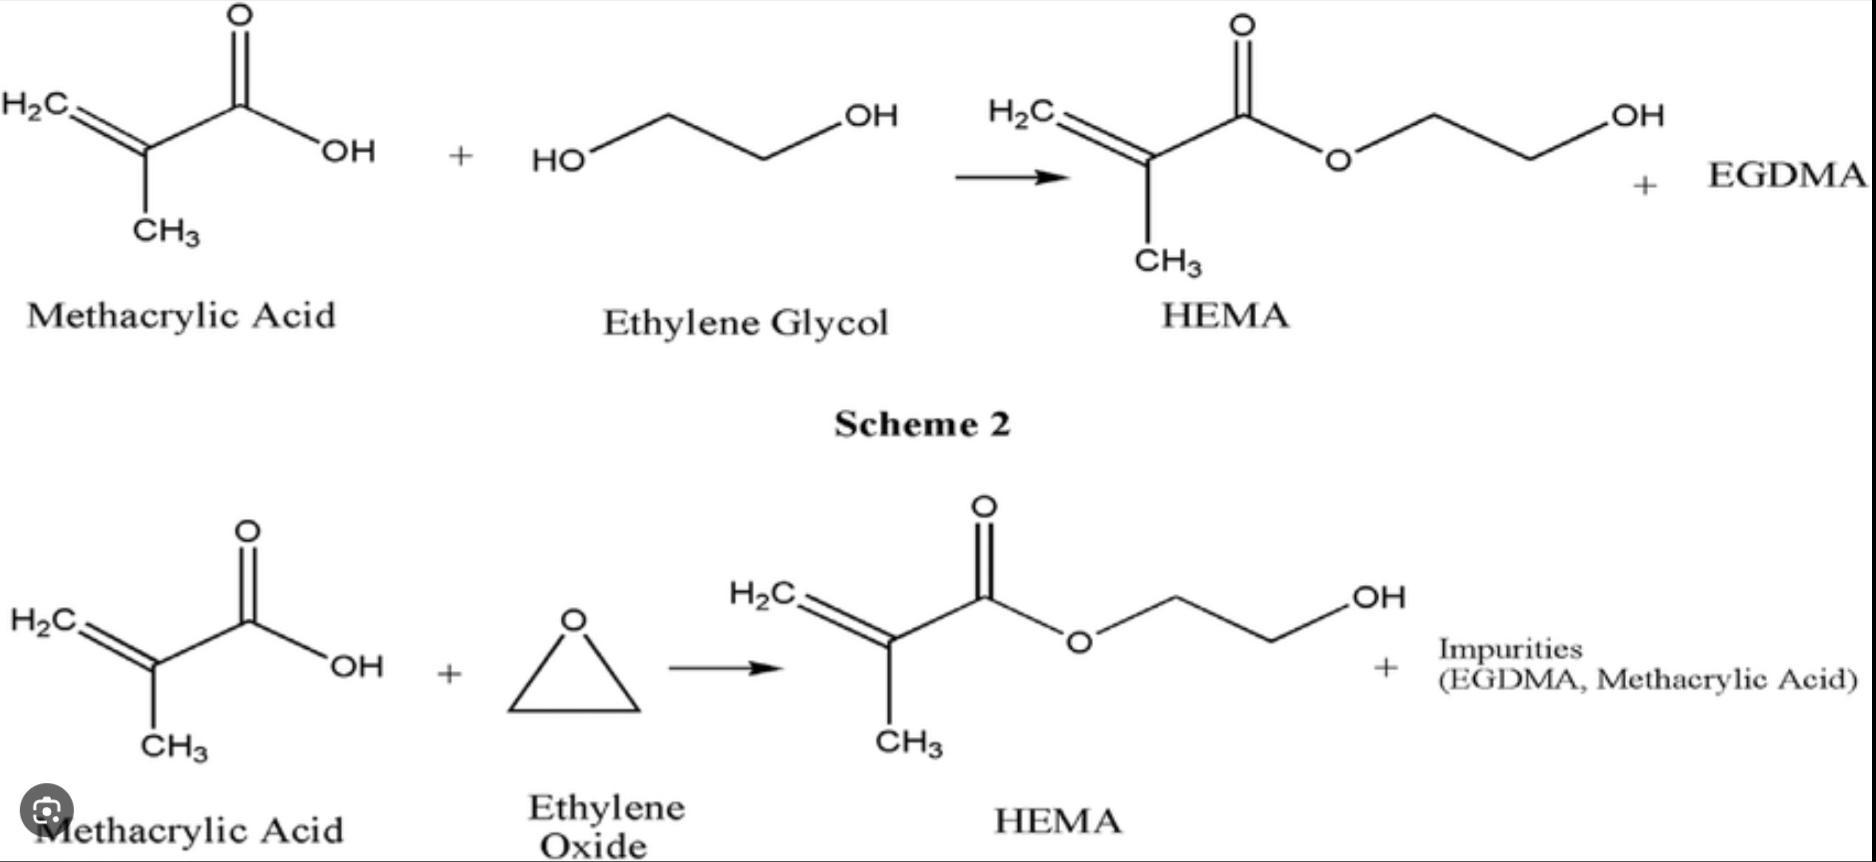
\includegraphics[width=12cm, height=10cm]{figures/screenshot001}
	\caption{Reaction routes to synthesize HEMA (make on your own)}
	\label{fig:hysteresis}
\end{figure}

\section{Comparison of the two processes}
In Table \ref{tab::hysteresis}, we can find an overall comparison of both the reactions. Reacting MAA with either EO and EG are both simple reactions. Reaction of MAA with EG uses an ion-exchange resin as a catalyst which enables and easy separation from bi-products. However it is equilibrium limited and the side-product EGDMA may react with the desired product to form a co-polymer. The formation of water is undesirable since HEMA is highly soluble in water. Water also promotes the polymerization of MAA. 

Reaction of MAA with EO is a more desirable choice as it is a direct one step synthesis, without any need for purification based on the purity of the MAA fed to the reactor since there are no side products formed. This reaction can be conducted continuously as opposed to the reaction of MAA with EG. However ethylene oxide is a highly flammable, highly carcinogenic and reactive material. So this reaction requires a very controlled environment. If the pressures or temperatures deviate even a little, there is a very high chance of a runaway reaction and a very major accident. 
\begin{table}[H]
	\centering
	\begin{tabular}{|p{3cm}|p{4cm}|p{4cm}|}
		\hline
		Process Variable & Esterification Reaction & Epoxidation Reaction \\
		\hline
		Pressure & Atmospheric Pressures & Vacuum of -0.99 – -0.75 Bar \\
		\hline
		Temeprature & 100-120 ℃ & 75 -90 ℃ \\
		\hline
		Catalyst & P-methyl benzene sulfonic acid or ion exchange catalysts & Ferric chloride immobilized on poly-acid \\
		\hline
		Reagent & Sulphuric acid & Tertiary amine such as pyridine, N,N-Dimethyl toluene etc. \\
		\hline
		Reaction time & 1 – 3 hr & 1.5 – 2 hr \\
		\hline
		Percentage yield & > 85\% & > 99\% \\
		\hline
		Polymerization inhibitor & Phenothiazine & MEHQ (hydroquinone monomethyl ether) \\
		\hline
		Impurities & Ethylene glycol dimethacrylate, Water & Ethylene glycol dimethacrylate \\
		\hline
	\end{tabular}
	\caption{Comparison of syntheses routes for HEMA}
	\label{tab::hysteresis}
\end{table}

\section{Comparison of the routes based on economic potential}
Economic potential(EP) is essentially the net difference between the price of the raw materials and the product. It can be used to compare the economic feasibility of two reactions to synthesize a chemical product.
It is given by the following formula;
$$ EP = Cost \ of \ desired \ Product \ per \ mole - Cost \ of \ Raw \ material \ Product \ per \ stochiometric \ moles $$

So if a desired product \textbf{P} is synthesized by the reaction 
$$ aA + bB \rightarrow P $$
and say cost of P is Rs X per mole, say cost of A is Rs Y per mole and say cost of b is Rs Z per mole, then the economic potential of this reacation will be 
$$ EP = X -(aY + bZ) $$
The route with more EP is more feasible. Table \ref{tab::hysteresis}, gives the price for synthezising HEMA using route 1 (using EG)
\begin{table}[H]
	\centering
	\begin{tabular}{|c|c|c|c|c|}
		\hline
		\textbf{Chemical} & \textbf{Moles in the reaction}	
		& \textbf{Molecular Weight} & \textbf{Price/kg (Rs.)} & \textbf{Price/mole (Rs.)} \\
		\hline
		EG & 1 & 62 & 65 & 4.03 \\
		\hline
		MAA & 1 & 86 & 150 & 12.9 \\
		\hline
		Water & 1 & 18 & 0 & 0 \\
		\hline
		HEMA & 1 & 130 & 160 & 20.8 \\
		\hline
	\end{tabular}
	\label{tab::hysteresis}
	\caption{Prices of the required chemicals to make HEMA using route 1 obtained from Chemical Weekly Buyers' Digest}
\end{table}	


Using these values, for this reaction, 

\begin{center}
	\textit{EP = 20.8-12.9-4.03}
	
	
	\textit{\textbf{EP = 3.87} }
\end{center}

In table \ref{tab::hysteresis}, the prices for the chemicals used to synthesize HEMA using route 2 (Ethylene Oxide) are given.

\begin{table}[h]
	\centering
	\begin{tabular}{|c|c|c|c|c|}
		\hline
		\textbf{Chemical} & \textbf{Moles} & \textbf{MW} & \textbf{Price/kg (in Rs)} & \textbf{Price/mole (in Rs.)} \\
		\hline
		EO   & 1 & 44  & 86  & 3.784 \\
		\hline
		MAA  & 1 & 86  & 150 & 12.9 \\
		\hline
		HEMA & 1 & 130 & 160 & 20.8 \\
		\hline
	\end{tabular}
	\label{tab::hysteresis}
	\caption{Prices of the required chemicals to make HEMA using route 2 obtained from Chemical Weekly Buyers' Digest}
\end{table}

Using these values, for this reaction 
\begin{center}
	\textit{EP = 20.8-12.9-3.78} 
	
	
	\textit{\textbf{EP = 4.12}}
\end{center}		

\subsection{Final selection of the process}
Based on the factors such as economic potential, raw materials used, yield, selectivity and the reaction conditions, the epoxidation route is more feasible for bulk production of HEMA. This route is also preferred globally. 

\chapter{Production of Methacrylic acid}


% === REFERENCES ===
\addcontentsline{toc}{chapter}{References}
\bibliographystyle{apacite}
\bibliography{references}




% === NOMENCLATURE (if needed) ===

\end{document}